\section{System's Perspective}
\begin{comment}
A description and illustration of the:

    Design and architecture of your ITU-MiniTwit systems
    All dependencies of your ITU-MiniTwit systems on all levels of abstraction and development stages. That is, list and briefly describe all technologies and tools you applied and depend on.
    Important interactions of subsystems.
        For example, via an illustrative UML Sequence diagram that shows the flow of information through your system from user request in the browser, over all subsystems, hitting the database, and a response that is returned to the user.
        Similarly, another illustrative sequence diagram that shows how requests from the simulator traverse your system.
    Describe the current state of your systems, for example using results of static analysis and quality assessments.


MSc students should argue for the choice of technologies and decisions for at least all cases for which we asked you to do so in the tasks at the end of each session.
^^^ 
^^^
\end{comment}

\subsection{Design \& Architecture}
\label{sec:design-architecture}

This section explains the overall structure, design decisions, and internal interactions of \emph{MiniTwitFS}, which consists of two top-level applications:

\begin{itemize}
  \item \textbf{MiniTwitAPI} – an ASP.NET Core Web API that exposes functions that talks to our Database.
  \item \textbf{MiniTwitClient} – a Blazor WebAssembly Application that runs entirely in the browser and communicates with the API.
\end{itemize}
The system implements a simplified Twitter-style micro-blog (“MiniTwitFS”)
where users can publish short messages, follow one another in
real time, and view their own timelines.

%---------------------------------------------------------------------------
\subsubsection{Architectural Style}

\begin{description}
  \item[Single-Page Client]  
        The Blazor WebAssembly front-end is downloaded once and
        then runs entirely in the browser. Navigation and state changes are
        handled client-side, so the UI behaves as a Single Page Application (SPA).

  \item[REST\,+\,\textit{occasional} SignalR]  
        All operations (e.g. \verb|/msgs|, \verb|/follows|, timeline
        queries) are standard REST requests over HTTPS. SignalR is currently used only for a secondary channel that streams live log messages to a developer page.

  \item[API Structure]  
        Inside \textbf{MiniTwitAPI} the code is organised as different layers.
        \emph{Presentation} (controllers and hubs)  
        $\rightarrow$ \emph{Application} (DTOs, use-case services)  
        $\rightarrow$ \emph{Domain} (entities, business rules)  
        $\rightarrow$ \emph{Infrastructure}.  
        Each layer has no compile-time dependency on an outer layer. All infrastructure (MySQL via EF Core, Serilog logging, authentication) is provided through dependency injection at startup.
\end{description}

%---------------------------------------------------------------------------
\subsubsection{High-Level Component View}

\begin{figure}[H]
    \centering
    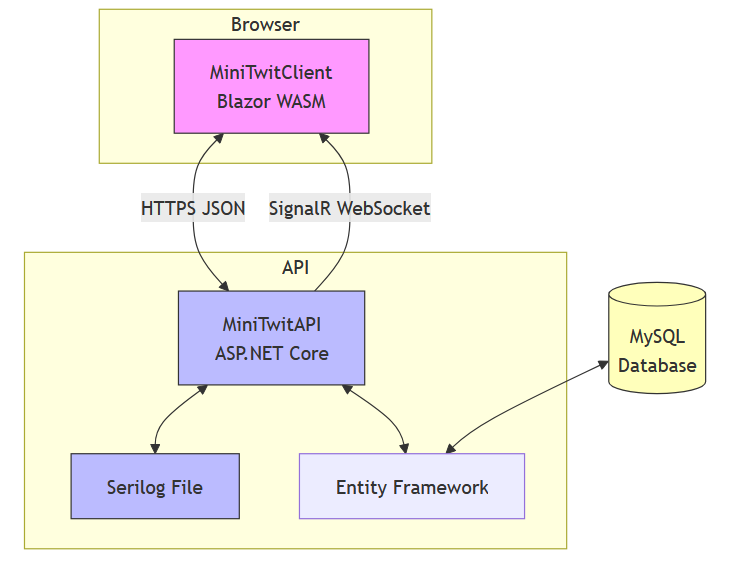
\includegraphics[width=1\linewidth]{images/Architecture.png}
    \caption{System Architecture}
    \label{fig:architecture}
\end{figure}

\paragraph{Explanation} MiniTwitClient communicates with the API through CORS-enabled HTTPS endpoints, authenticating with JSON Web Tokens (JWT). When a user posts a new message, the API stores the record in the database and broadcasts a \emph{\lstinline{MessageAdded}} event over SignalR. Connected
admin clients update their logs instantly without refreshing the page. See Figure \ref{fig:architecture} for a visualization.

%---------------------------------------------------------------------------
\subsubsection{Internal Structure of \texttt{MiniTwitAPI}}

\begin{itemize}
  \item \textbf{Controllers}  
        Request endpoints that validates input and implements use-cases such as
        \lstinline{PostMessage}, \lstinline{FollowUser}, and
        \lstinline{GetTimeline}.
  \item \textbf{Domain Models}  
        Database Entities: \lstinline{User}, \lstinline{Message}, and
        \lstinline{Follower}. Also DTO's and request models, e.g. AddMessageRequest and LoginRequest.
  \item \textbf{Infrastructure}  
        \lstinline{AppDbContext} (EF Core with migrations), JWT authentication middleware, ILogger and SignalR.
  \item \textbf{Configuration}
The base \textit{appsettings.json} is overridden by \textit{appsettings.Development.json} or \textit{appsettings.Production.json} according to the DOTNET\_ENVIRONMENT variable.

The database connection string, JWT signing key and the simulator’s Basic-auth header are \emph{not} checked into Git, instead they are injected at runtime via DigitalOcean “App secrets”.

Injections, mappings, authentication, and different services and rules, are all setup on startup through the \textit{Program.cs} file. 

The migration command is executed on production release as part of the release pipeline, in order to guarantee that the runtime database schema always matches the current code.

Serilog logs are written to the console during development and to DigitalOcean’s log stream in production, driven by the \textit{Serilog:WriteTo} section.
\end{itemize}

Figure \ref{fig:apicontrollerclass} shows a class diagram of the API MinitwitController.

\begin{figure}[H]
    \centering
    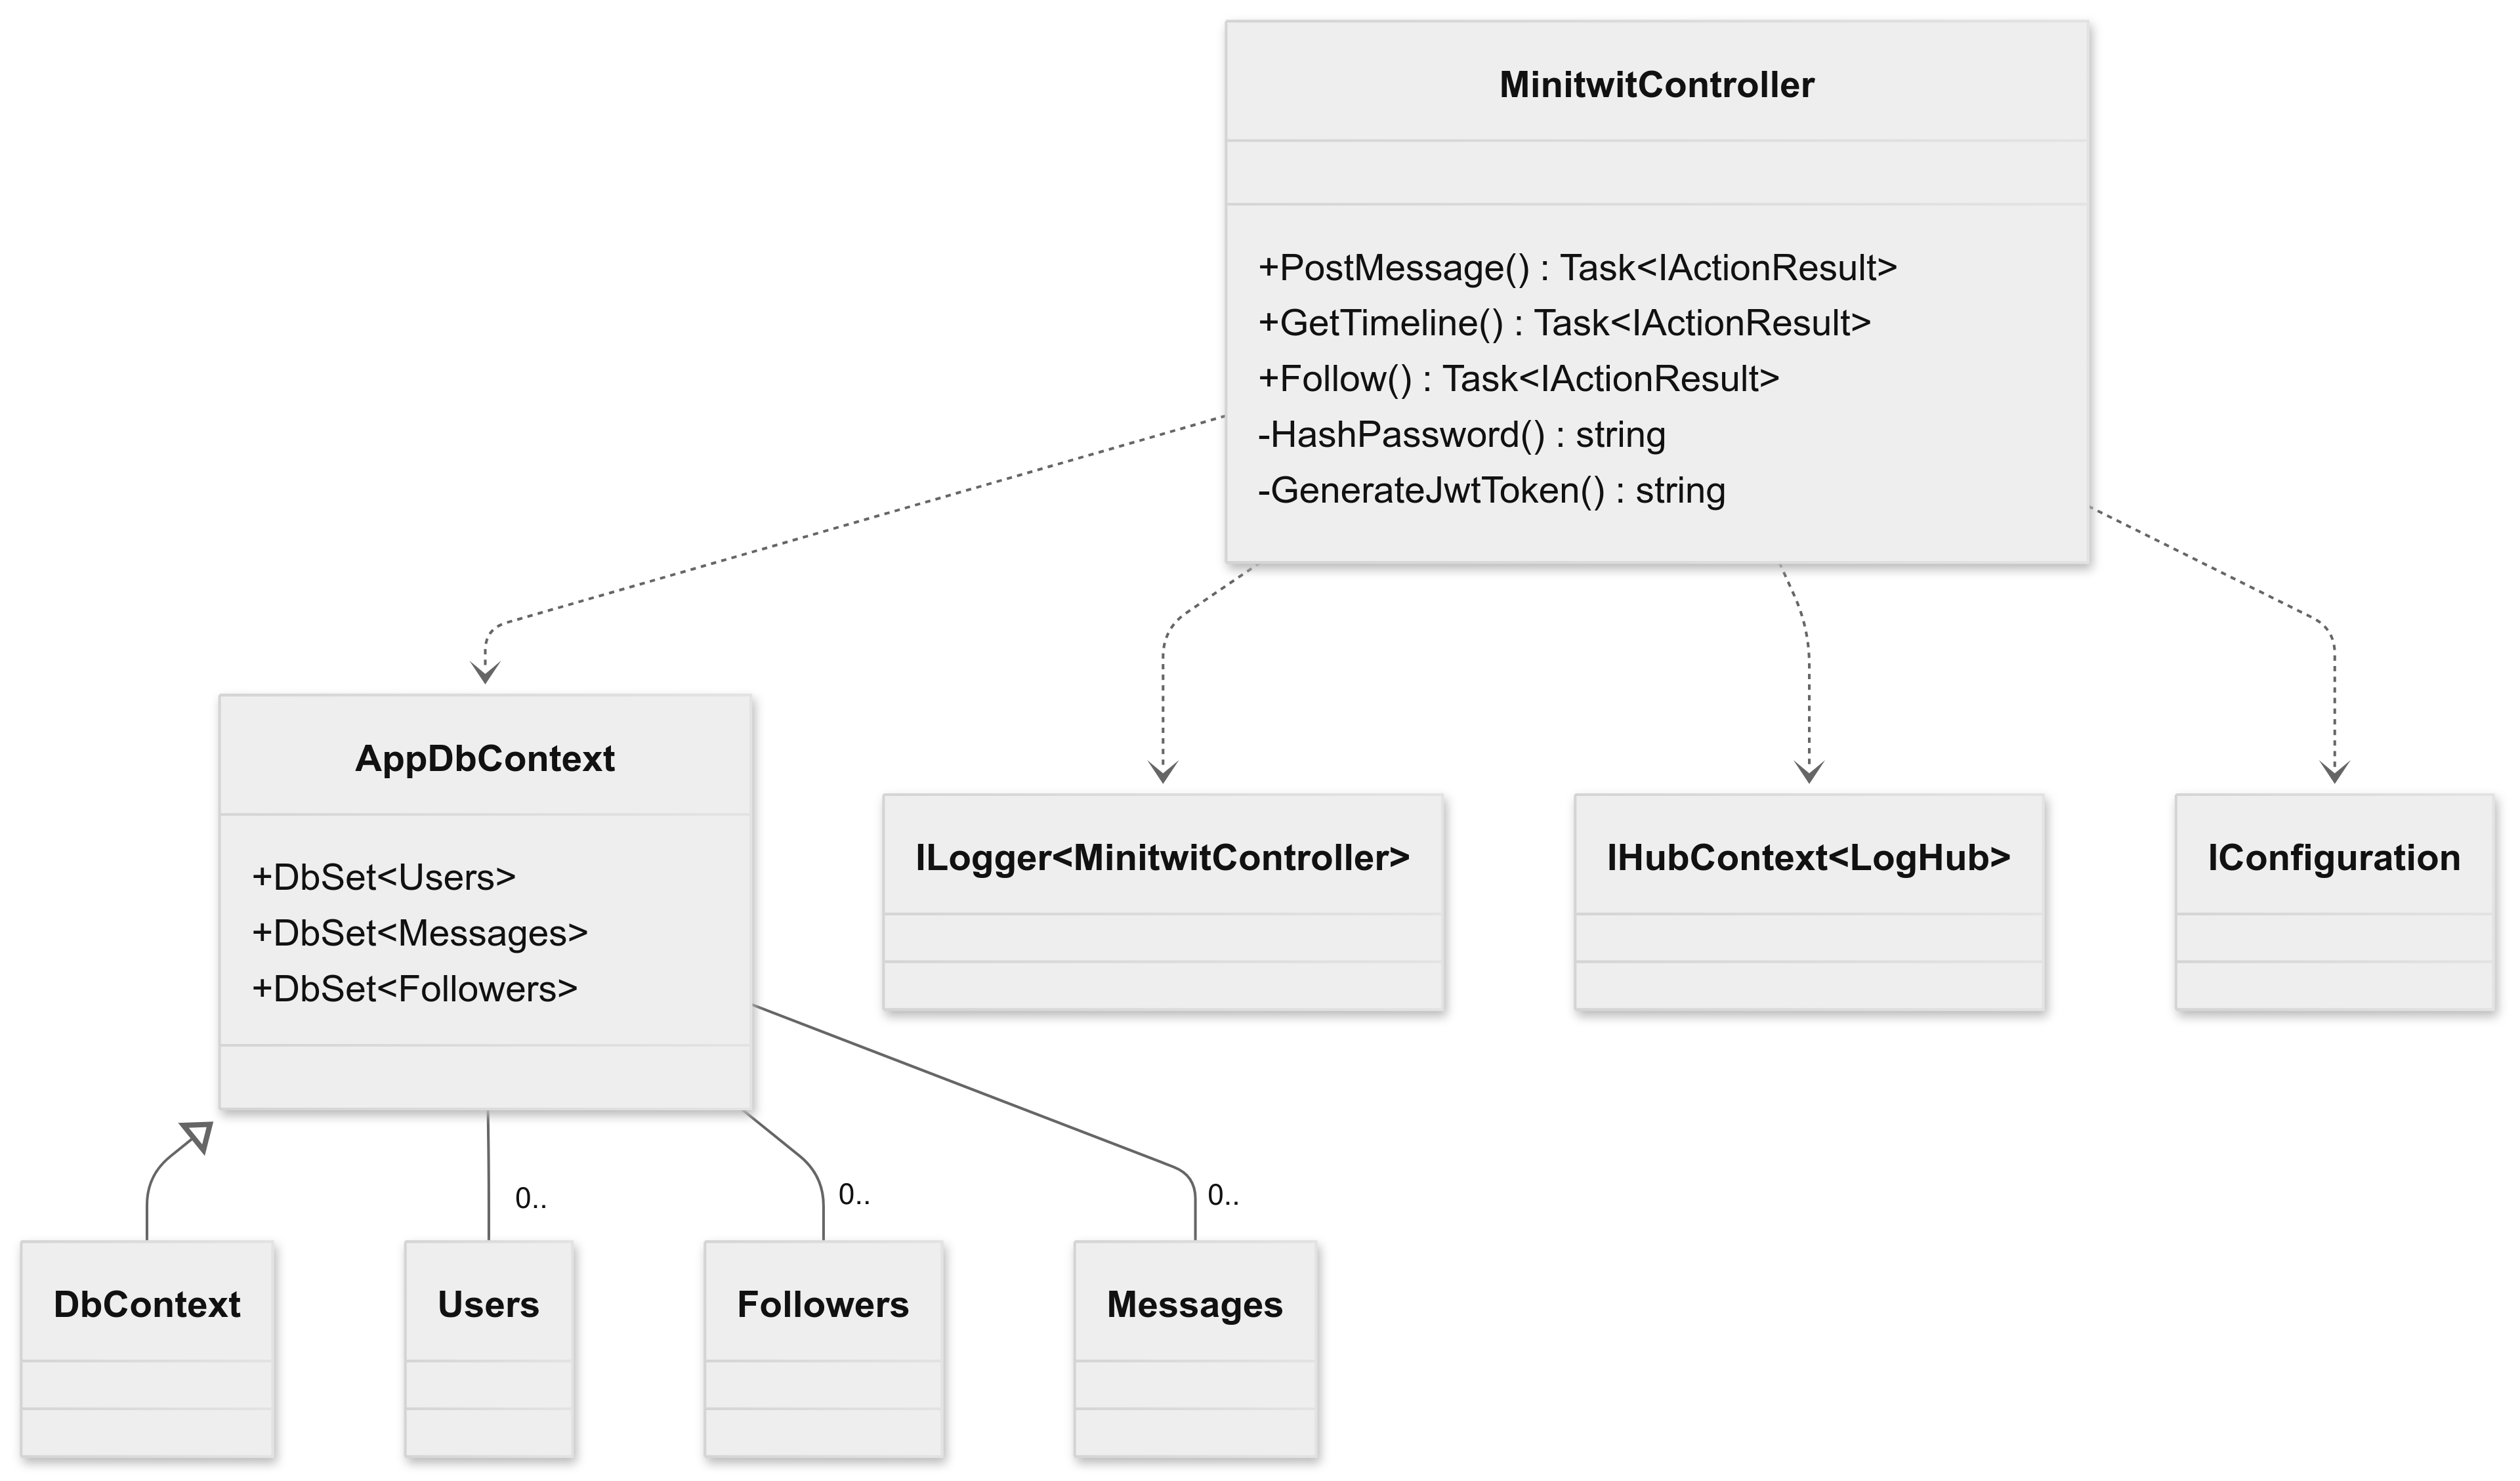
\includegraphics[width=1\linewidth]{images/APIClass2.png}
    \caption{Class diagram of MinitwitController in the API}
    \label{fig:apicontrollerclass}
\end{figure}

%---------------------------------------------------------------------------
\subsubsection{Internal Structure of \texttt{MiniTwitClient}}

The client is compiled from C\# Razor components to WebAssembly.  A
lightweight state–container service called \lstinline{UserState} keeps the currently authenticated user (name and JWT). Components inject this service and read its properties.

\begin{itemize}
  \item \textbf{Pages}  
        \lstinline{/register}, \lstinline{/login}, \lstinline{/public},
        \lstinline{/timeline}, \lstinline{/user/username}.
  \item \textbf{Shared Components}  
        NavMenu, MessageCard, FollowButton, and toast notifications.
  \item \textbf{Services}  
        \lstinline{MinitwitController} (typed REST client),
        optional \lstinline{WebSocketService} for live log streaming,
        Tailwind CSS for styling, and small JS-interop helpers.
  \item \textbf{Configuration}
The HTML page sets a window.appConfig.apiEndpoint value, where the Blazor code reads that value through JavaScript interop, so the same build of the site works in every environment without being rebuilt. It is setup so that the value gets overwritten both when running locally, or when built in the pipeline, with the correct values - controlled by the project settings.

If the user has logged in, the generated JSON Web Token is stored in sessionStorage. When the page reloads the token is re-read, and, if it is present, a Bearer header is attached to every HTTP request.

Tailwind CSS compiles the code into an index.html, and bundled CSS files, when pushing to production;
\begin{quote}
    \textit{Tailwind automatically removes all unused CSS when building for production, which means your final CSS bundle is the smallest it could possibly be.} \cite{tailwind}
\end{quote}

\end{itemize}

Figure \ref{fig:ClientClass} shows a class diagram example from the client.

\begin{figure}[H]
    \centering
    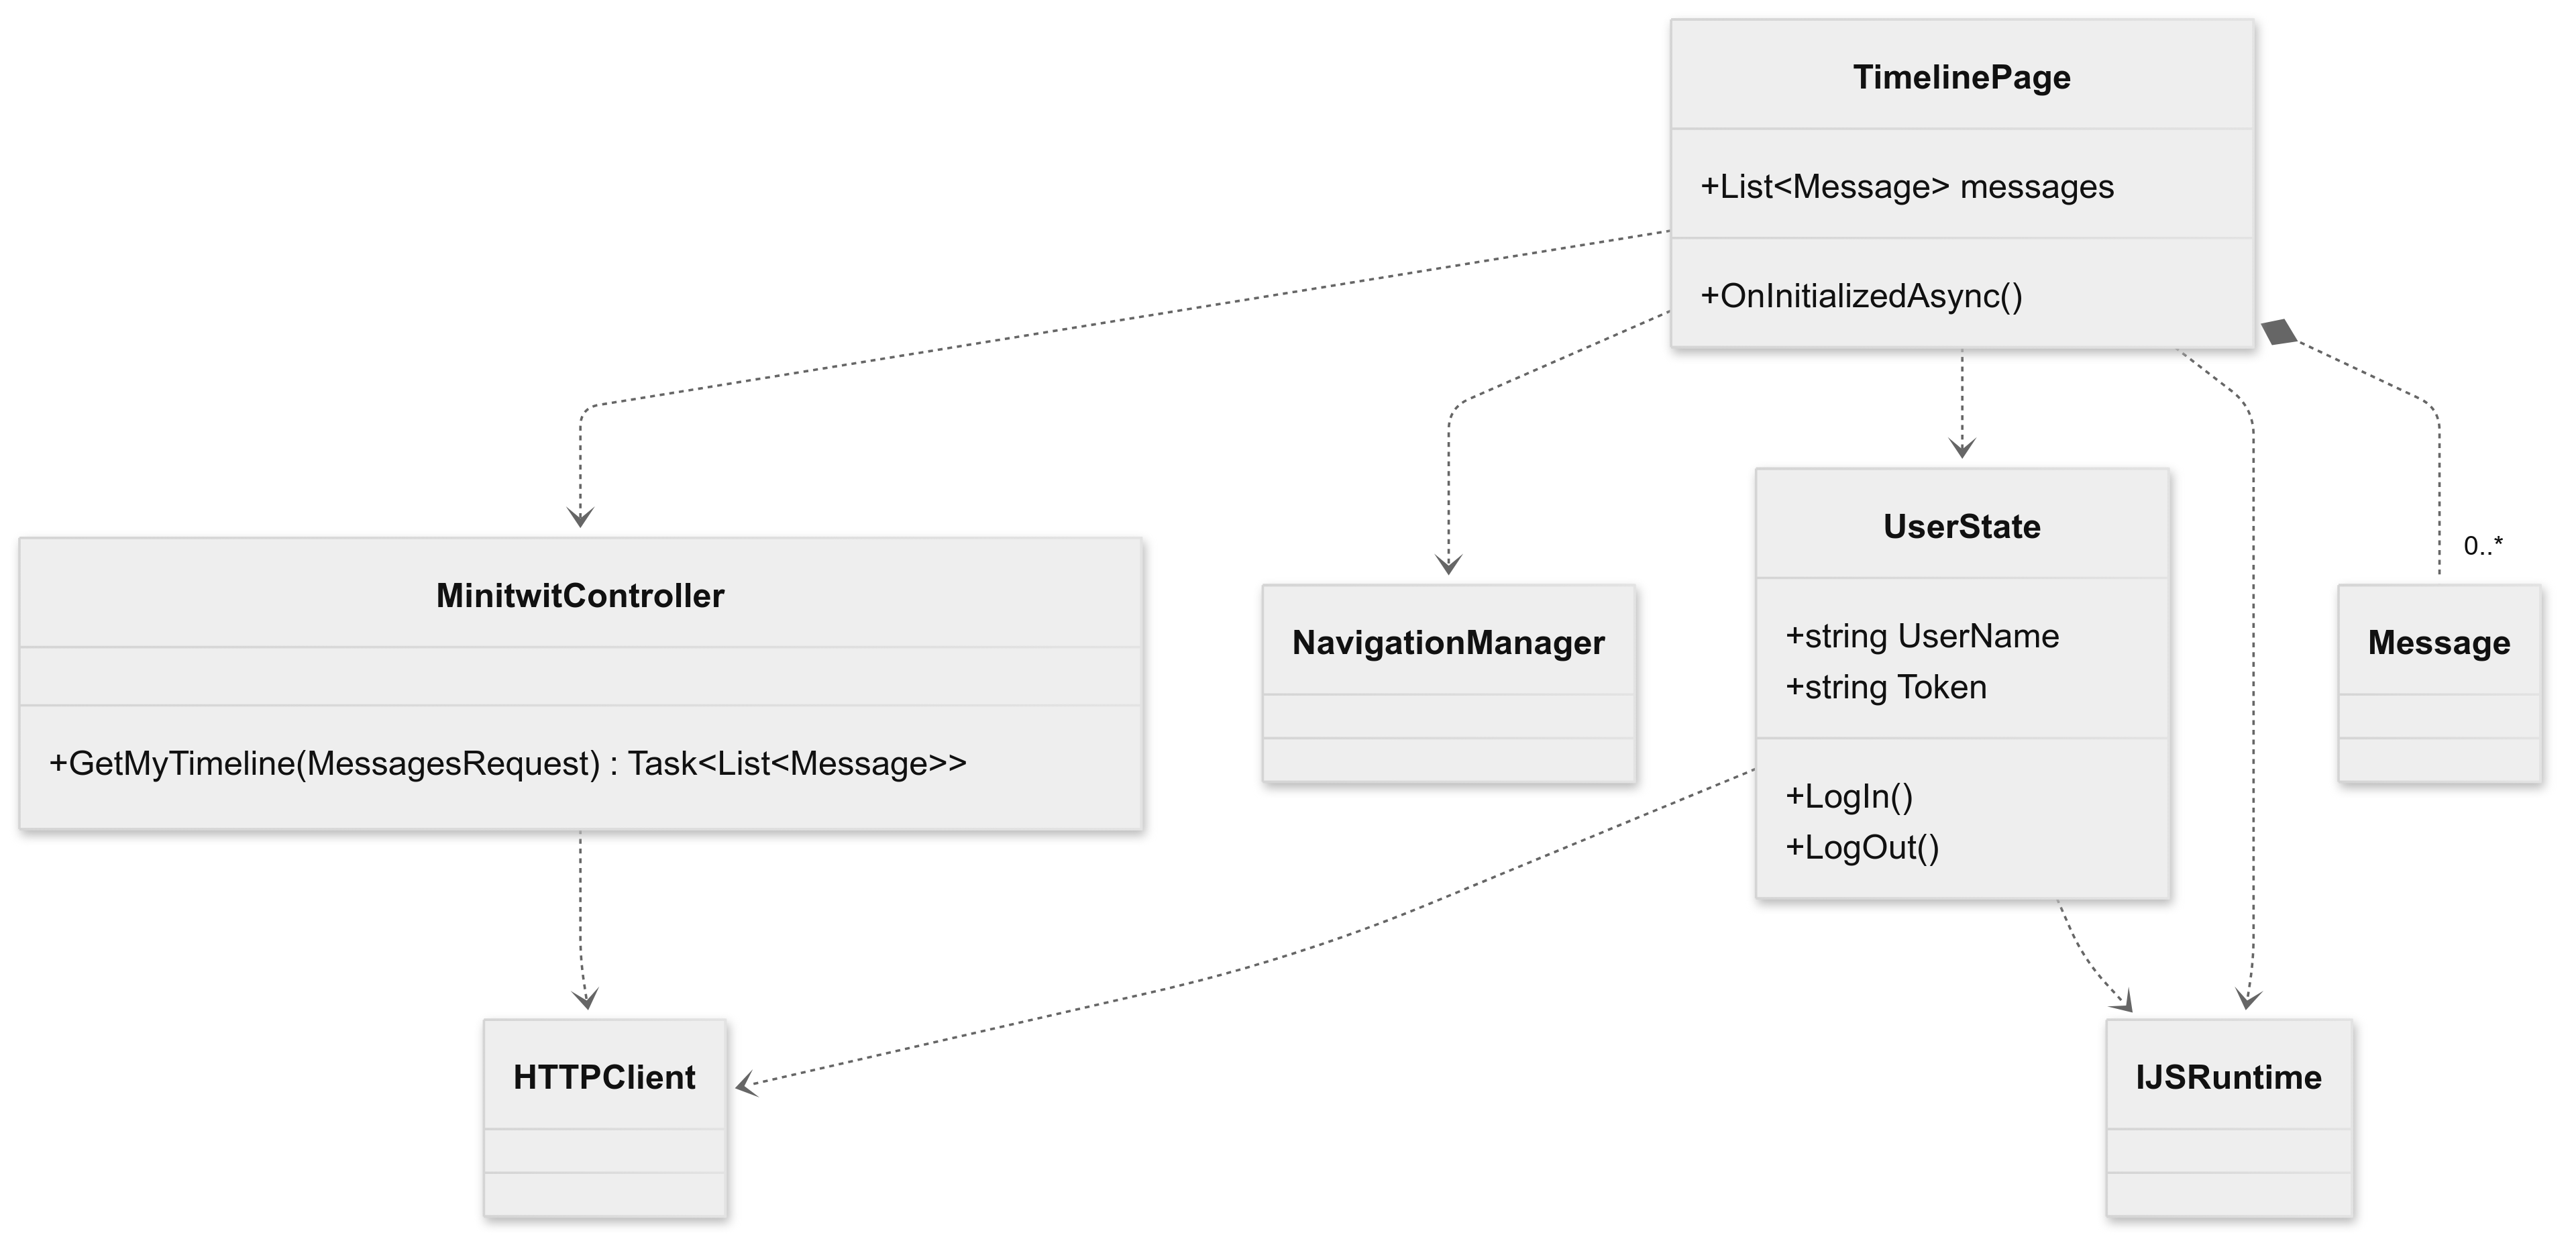
\includegraphics[width=1\linewidth]{images/ClientClass2.png}
    \caption{Class diagram of Timeline page}
    \label{fig:ClientClass}
\end{figure}

%---------------------------------------------------------------------------
\subsubsection{Typical Runtime Interactions}
When a real user wants to interact with our system, they do so through our web client. Here, the user is restricted by the user interface we have provided, however the requests that the user does still goes through all of the systems.

Figure \ref{fig:runtimeseq} shows a sequence diagram, depicting the different calls between systems, in a successful post-message request from the client.

\begin{figure}[H]
    \centering
    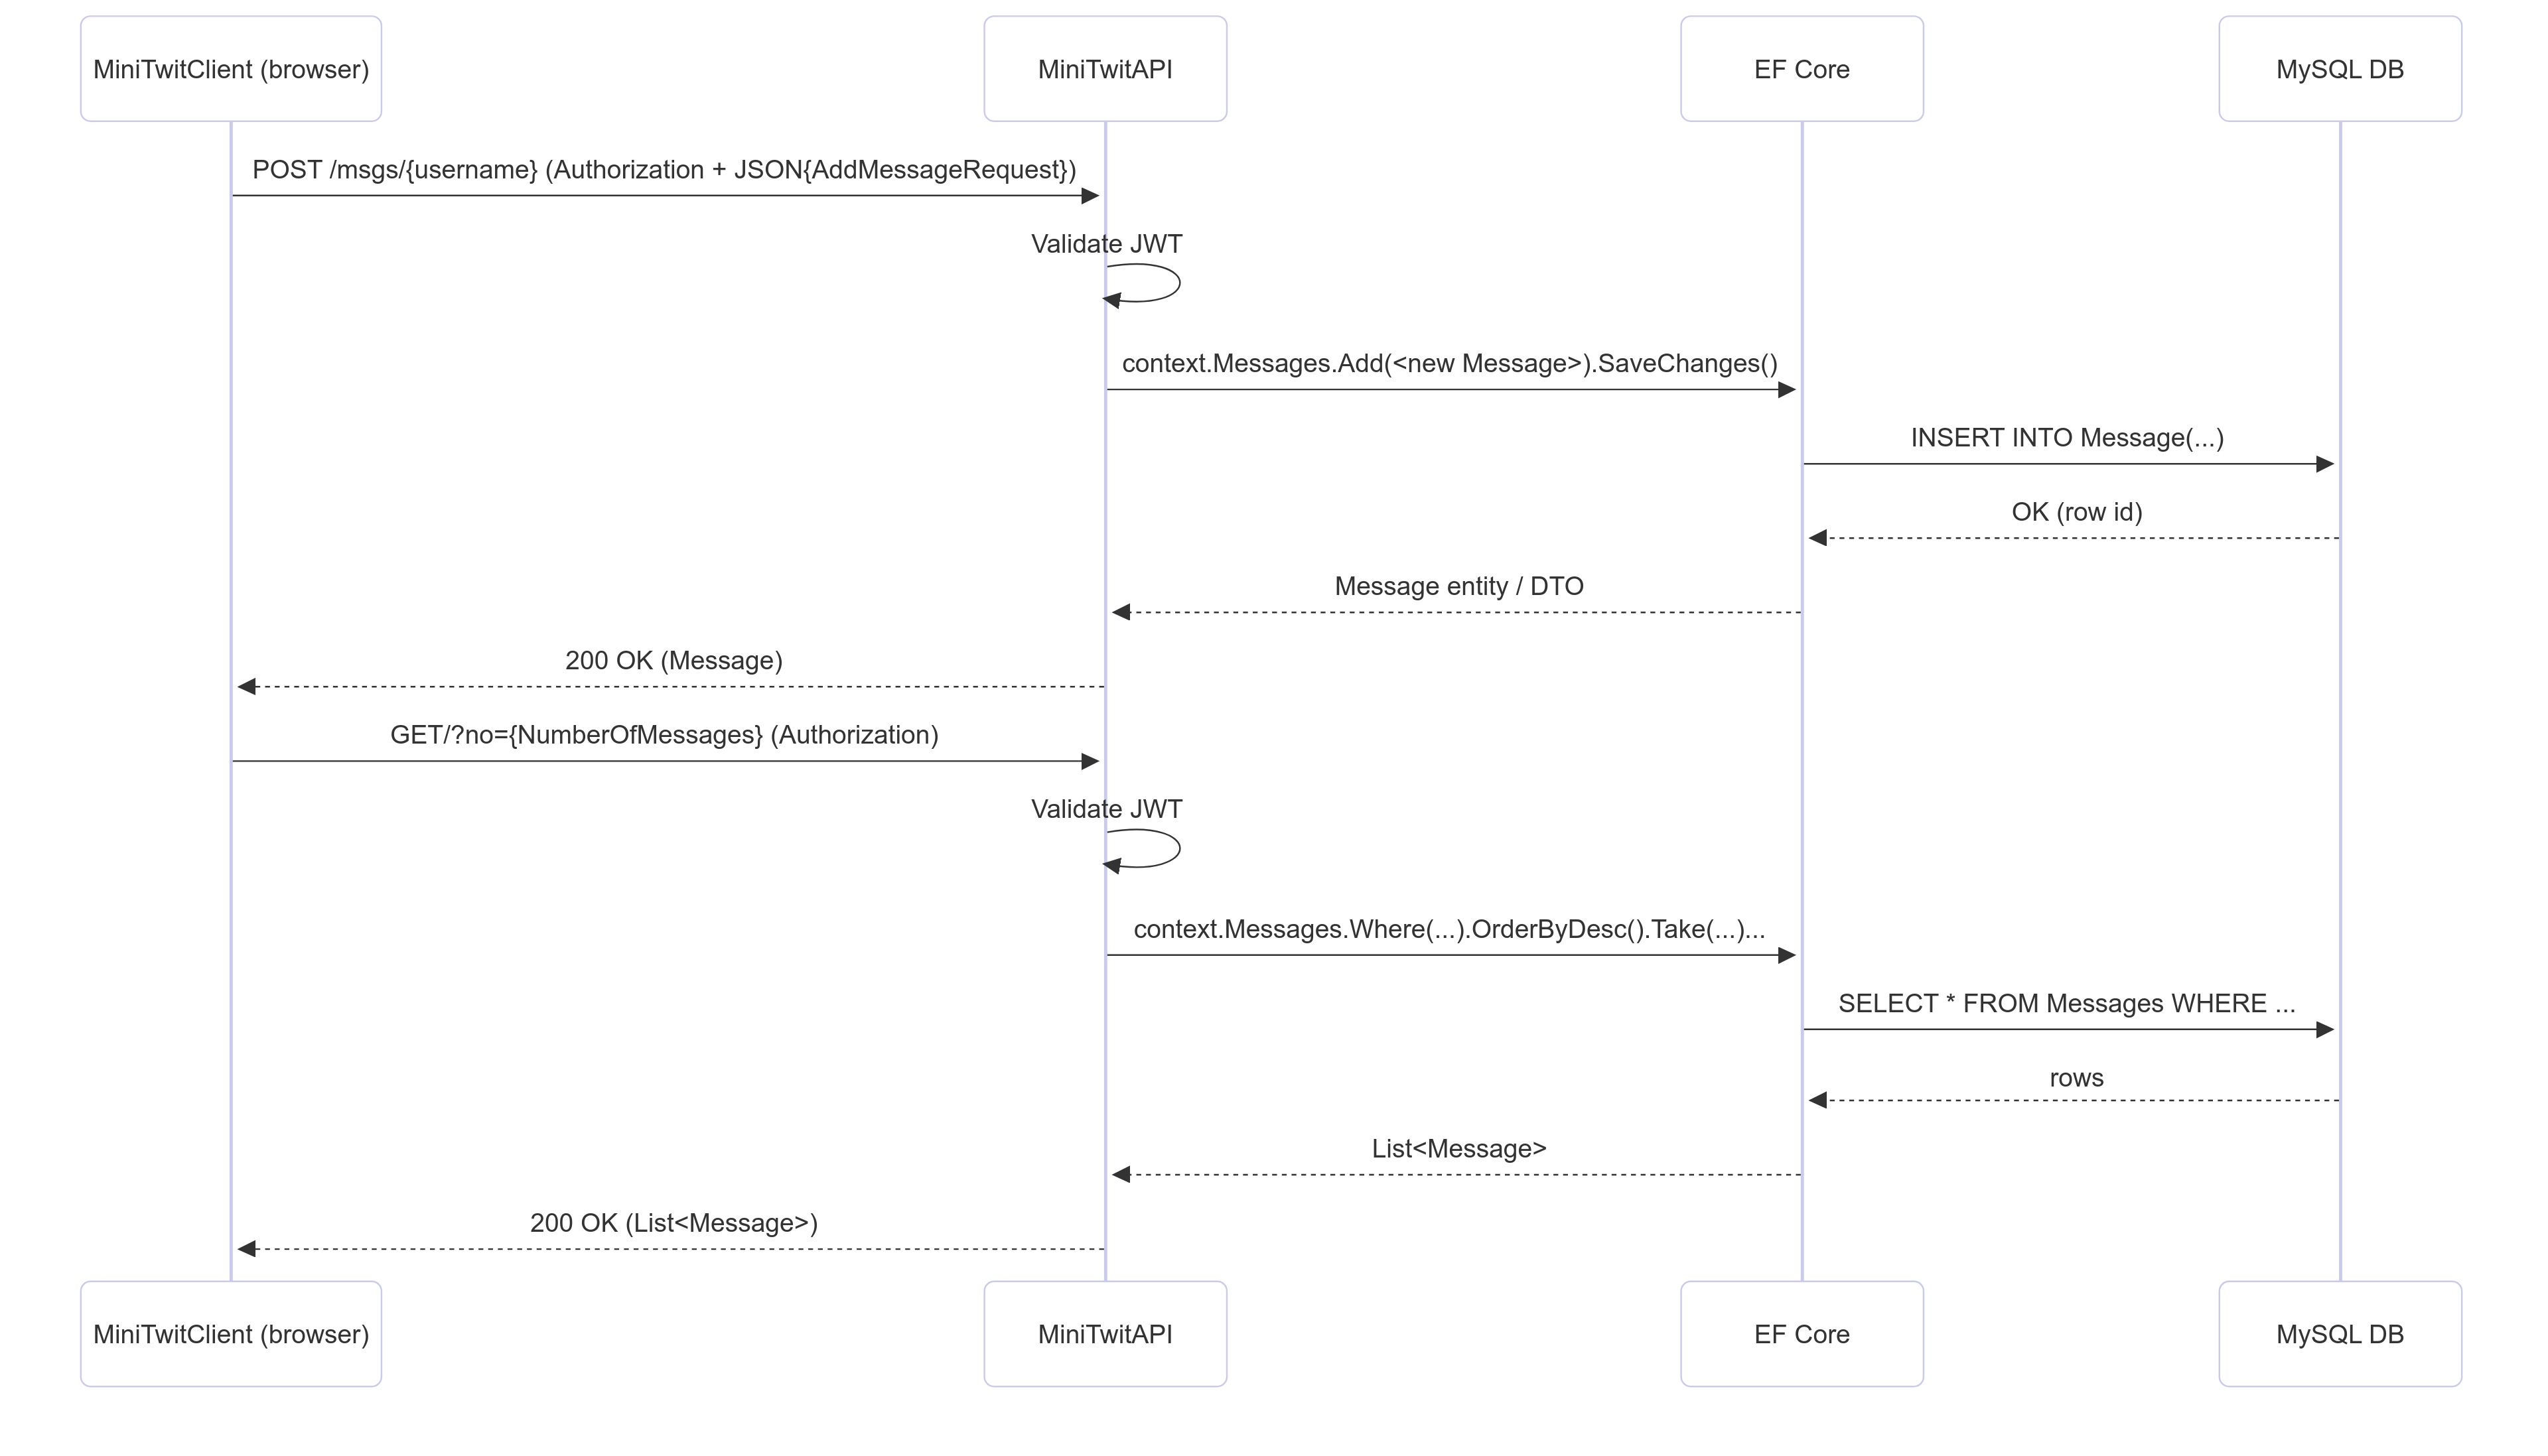
\includegraphics[width=1\linewidth]{uml/Editor _ Mermaid Chart-2025-05-28-100914.png}
    \caption{Client doing post request to the API, and the response they receive}
    \label{fig:runtimeseq}
\end{figure}

However, the simulator connects directly to the API, uses a Basic authorization header, and doesn't use the response, which can be seen in figure \ref{fig:SimSeq2}.

\begin{figure}[H]
    \centering
    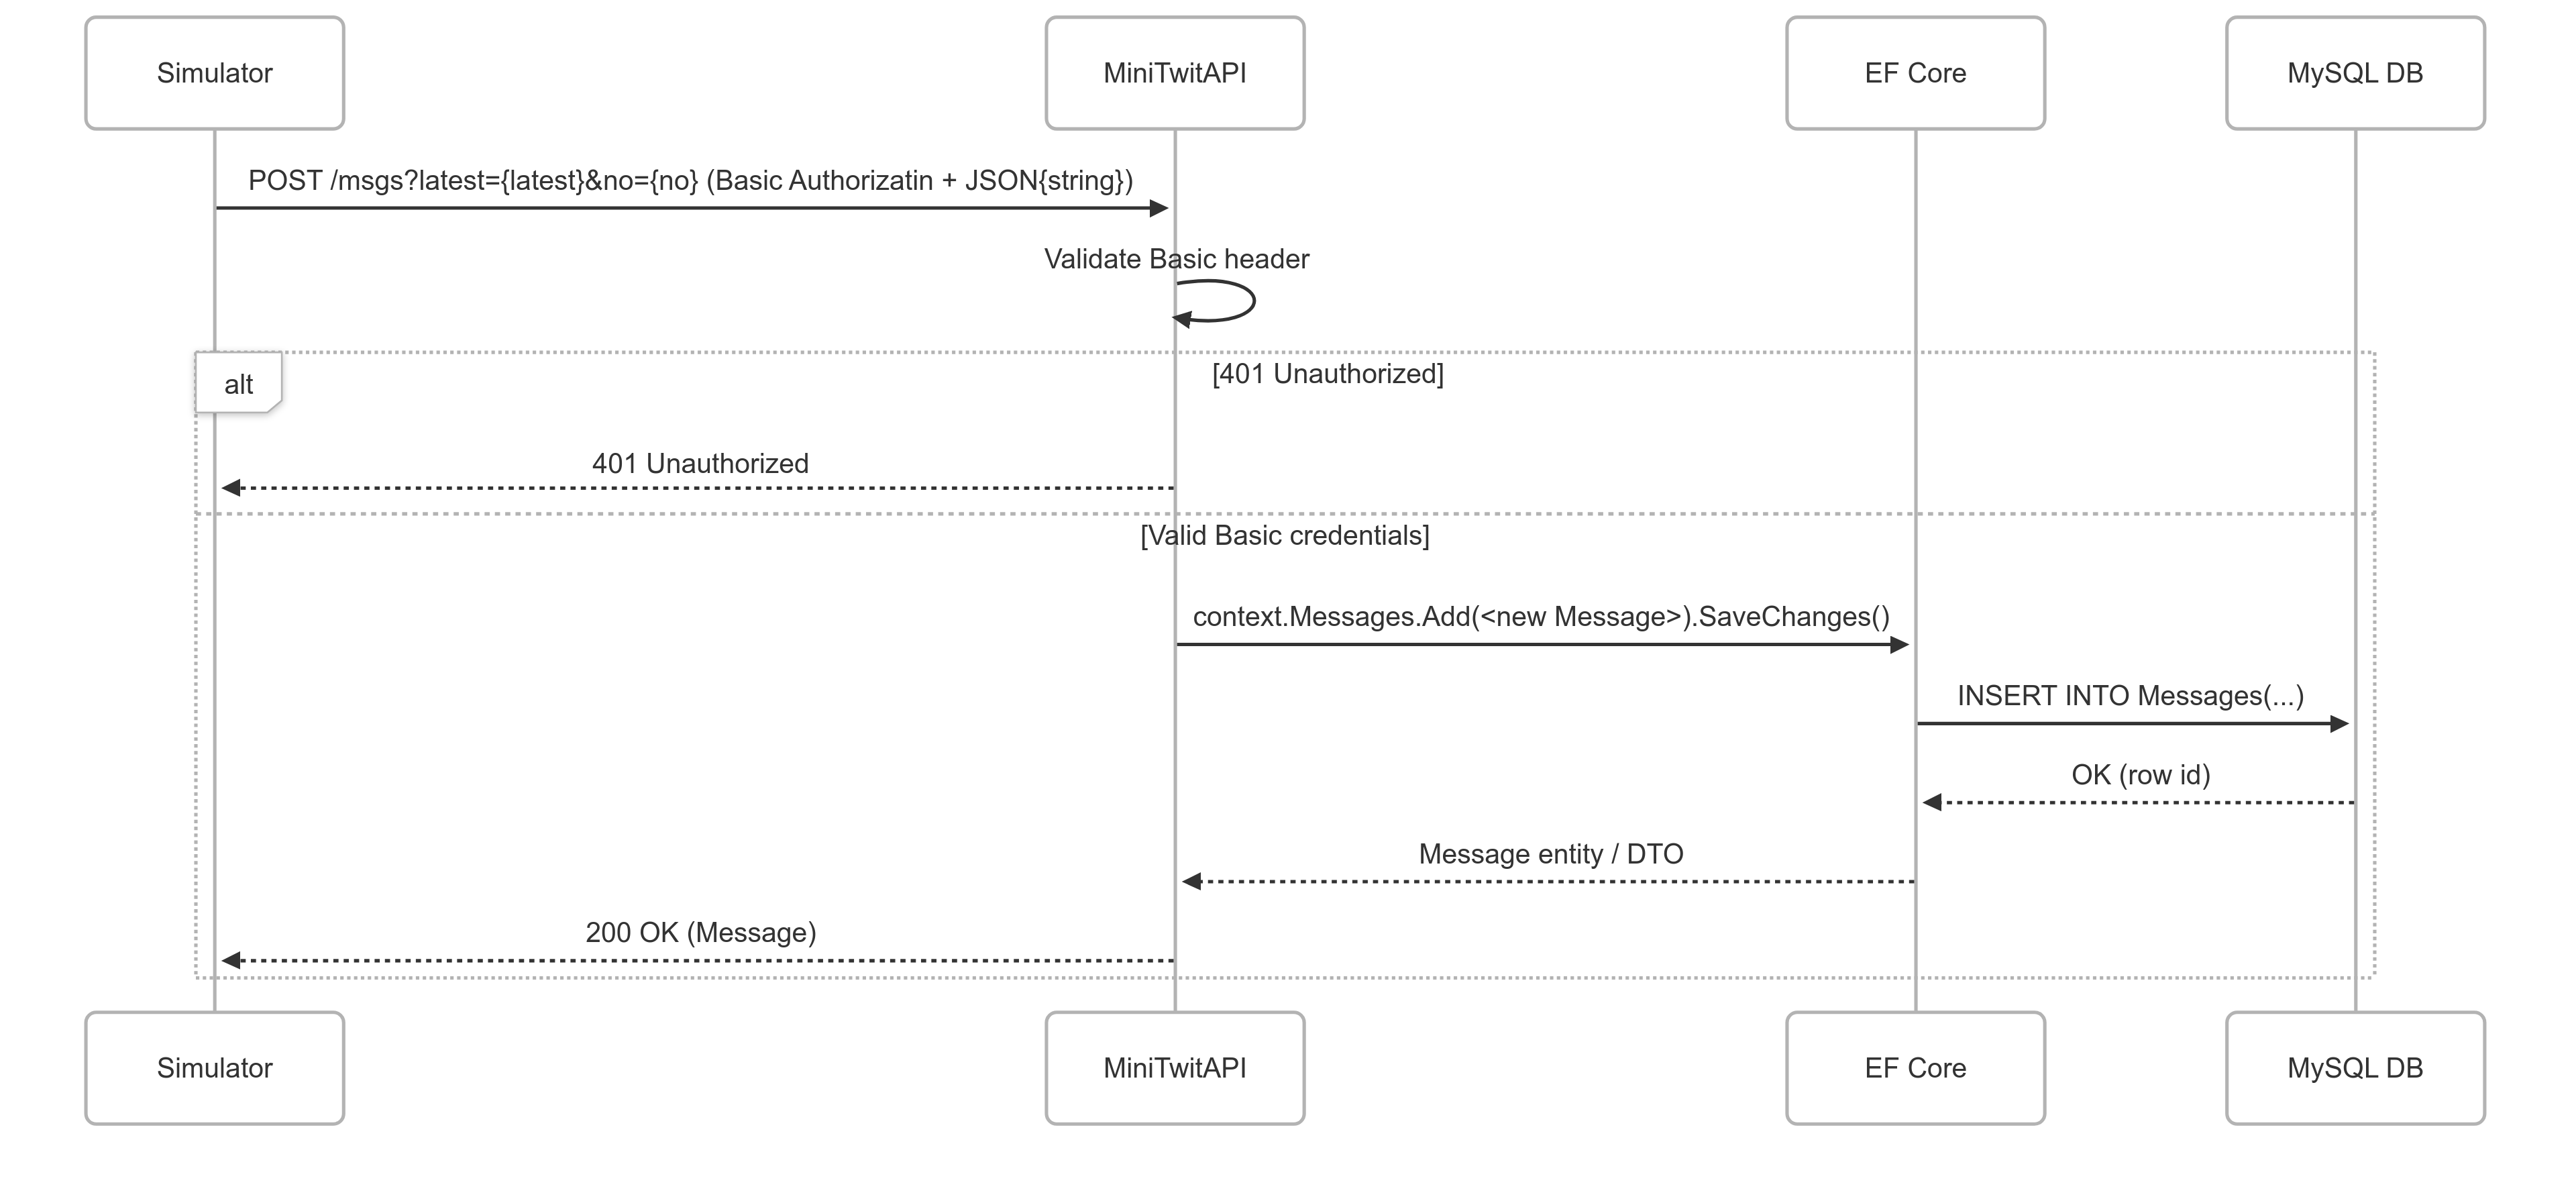
\includegraphics[width=1\linewidth]{images/SimSeq2.png}
    \caption{Simulator doing post request to the API}
    \label{fig:SimSeq2}
\end{figure}

%---------------------------------------------------------------------------
\subsubsection{Authentication \& Authorization - Current vs Target}
\label{sec:auth-current-target}

\paragraph{Current implementation}
\begin{itemize}
  \item \textbf{Client users}  
        Receive a JSON Web Token (JWT) at login. Defaults to Simulator Basic authorization when not logged in. All requests
        carry the current token.
  \item \textbf{Simulator}  
        Uses a hard-coded Basic auth header that is accepted by a custom middleware.
  \item \textbf{Endpoint protection.}  
        Controllers are simply decorated with \verb|[Authorize]|, which
        validates the JWT; however, the middleware lets any request with
        the simulator Basic authorization pass, giving it the same privileges as a logged-in user.
\end{itemize}

\paragraph{Identified shortcomings}
\begin{itemize}
  \item The Basic credential leaks to every unauthenticated visitor via
        network traces.
  \item Any attacker who copies the header can post, follow, or delete
        on behalf of any user, e.g. through Postman.
\end{itemize}

\paragraph{Target implementation}
\begin{itemize}
  \item \textbf{No Basic fallback in the client.}  
        Anonymous browsers send \textbf{NO} Authorization header.
        Authenticated browsers sends a JWT only.
  \item \textbf{Dual authentication schemes.}  
        The API registers both
        \texttt{JwtBearer} (for browsers) and \texttt{SimulatorBasic}
        (for the simulator).  A dedicated handler validates the secret
        header and tags requests as \emph{simulator} for logging.
  \item \textbf{Explicit endpoint rules.}  
        Write actions are protected by something similar to 
        \verb|[Authorize(AuthenticationSchemes =|
        \verb| "Bearer, SimulatorBasic",|
        \verb| Policy = "UserMatchesRoute")]|
        meaning a request is allowed only when
        either a valid JWT whose subject matches the
        \texttt{\{username\}} route \emph{or} the simulator header is
        present.  Public GET endpoints are marked
        \verb|[AllowAnonymous]|.
\end{itemize}

\paragraph{Why this matters.}
Removing the Basic fallback closes the inadvertent back-door while still
letting the simulator operate.  Separate schemes enable clearer auditing,
future rate-limits, and rotation of the simulator secret without touching
user flows. Current setup is not secure at all.

\subsubsection{DigitalOcean Setup}
Our system is deployed on DigitalOcean using an IaaP App Platform where the API is configured as a web service and the client as a static site. The platform has a reference to our repository on GitHub, where the clients output directory looks for a build in the dist/wwwroot located in the MiniTwitClient project. Additionally, we have a MySQL database set up as well, which is attached to the platform, and the SnapShooter add-on to backup the database.

\subsection{Dependencies, Technologies \& Rationale}
All dependencies and technologies are shown on Table 1 and Table 2.
\begin{comment}
    \begin{itemize}
        \item \textbf{Microsoft ASP.NET Core~8 (Web API)}\cite{web-api-tutorial} – A framework for building RESTful web services using C\# and .NET. Compared to Node/Express, it provides static typing, built‑in dependency injection, and higher baseline throughput in Linux containers.
        
        \item \textbf{Entity Framework Core~8 (Code‑First)}\cite{Entity-Framework-Core} – An object–relational mapper that maps .NET objects to SQL tables and handles migrations. Compared to lightweight mappers like Dapper, its automatic migrations and LINQ queries remove boilerplate while still allowing raw SQL when required.
        
        \item \textbf{Blazor WebAssembly (stand‑alone)}\cite{blazor} – Runs C\# directly in the browser via WebAssembly with no JavaScript bundle. Compared to a React+TypeScript front‑end, it keeps the entire stack in one language and reuses existing DTOs.
        
        \item \textbf{SignalR}\cite{signalr} – Real‑time library that pushes server updates to clients over WebSockets or graceful fall‑backs. 
        
        \item \textbf{Tailwind CSS}\cite{tailwind} – A utility‑class framework applied directly in markup. Compared to Bootstrap, its purge step removes unused styles, shrinking the CSS bundle and keeping component markup concise.
        
        \item \textbf{Docker}\cite{docker} – Packages the app and its dependencies into containers, ensuring identical development and production environments. Compared to shell scripts on raw VMs, it eliminates “works on my machine” drift and enables one‑command integration test environments.
        
        \item \textbf{DigitalOcean}\cite{digitalocean} – Cloud provider offering computing, storage, and managed MySQL. We chose it over Azure and Google Cloud, because it was the only service we could get up and running successfully.
        
        \item \textbf{GitHub Actions}\cite{github_actions} – CI/CD that runs tests, lints, builds images, and deploys on every pull request. Compared to Jenkins, it requires no self‑hosted server or plugin maintenance.
        
        \item \textbf{MySQL}\cite{mysql} – Relational database engine powering production. Compared to PostgreSQL, the team already knew its tooling and DigitalOcean offers it as a fully managed service.
        
        \item \textbf{xUnit}\cite{xUnit} – Unit‑testing framework for .NET with a clean attribute syntax. Compared to MSTest or NUnit, it executes tests in parallel out of the box and integrates tightly with the .NET CLI.
        
        \item \textbf{Serilog}\cite{serilog} – Structured logging library that writes JSON to files, Seq, or Grafana/Loki. Compared to the default Microsoft logger, it produces queryable, schema‑less logs without extra adapters.
        
        \item \textbf{SnapShooter}\cite{snapshooter} – Backup service creating scheduled and on‑demand snapshots of volumes and databases. Compared to a hand‑rolled \texttt{mysqldump}+\emph{cron}, it handles retention policies and one‑click restores for us.
    \end{itemize}
\end{comment}

\begin{table}[H]
\centering
\begin{tabularx}{\linewidth}{@{}p{3cm}p{1.5cm}X@{}}
\toprule
\textbf{Technology} & \textbf{Citation} & \textbf{Description}\\
\midrule
Microsoft ASP.NET Core 8 (Web API) & \cite{web-api-tutorial} & A framework for building RESTful web services using C\# and .NET. Compared to Node/Express, it provides static typing, built-in dependency injection, and higher baseline throughput in Linux containers.\\\midrule
Entity Framework Core 8 (Code-First) & \cite{Entity-Framework-Core} & An object–relational mapper that maps .NET objects to SQL tables and handles migrations. Compared to lightweight mappers like Dapper, its automatic migrations and LINQ queries remove boilerplate while still allowing raw SQL when required.\\\midrule
Blazor WebAssembly (stand-alone) & \cite{blazor} & Runs C\# directly in the browser via WebAssembly with no JavaScript bundle. Compared to a React+TypeScript front-end, it keeps the entire stack in one language and reuses existing DTOs.\\\midrule
SignalR & \cite{signalr} & Real-time library that pushes server updates to clients over WebSockets or graceful fall-backs.\\\midrule
Tailwind CSS & \cite{tailwind} & A utility-class framework applied directly in markup. Compared to Bootstrap, its purge step removes unused styles, shrinking the CSS bundle and keeping component markup concise.\\\midrule
Docker & \cite{docker} & Packages the app and its dependencies into containers, ensuring identical development and production environments. Compared to shell scripts on raw VMs, it eliminates “works on my machine” drift and enables one-command integration test environments.\\
\bottomrule
\end{tabularx}
\caption{Technology stack with citations and rationale.}
\end{table}

\begin{table}[H]
\centering
\begin{tabularx}{\linewidth}{@{}p{3cm}p{1.5cm}X@{}}
\toprule
\textbf{Technology} & \textbf{Citation} & \textbf{Description}\\
\midrule
DigitalOcean & \cite{digitalocean} & Cloud provider offering computing, storage, and managed MySQL. We chose it over Azure and Google Cloud because it was the only service we could get up and running successfully.\\\midrule
GitHub Actions & \cite{github_actions} & CI/CD that runs tests, lints, builds images, and deploys on every pull request. Compared to Jenkins, it requires no self-hosted server or plugin maintenance.\\\midrule
MySQL & \cite{mysql} & Relational database engine powering production. Compared to PostgreSQL, the team already knew its tooling and DigitalOcean offers it as a fully managed service.\\\midrule
xUnit & \cite{xUnit} & Unit-testing framework for .NET with a clean attribute syntax. Compared to MSTest or NUnit, it executes tests in parallel out of the box and integrates tightly with the .NET CLI.\\\midrule
Serilog & \cite{serilog} & Structured logging library that writes JSON to files, Seq, or Grafana/Loki. Compared to the default Microsoft logger, it produces queryable, schema-less logs without extra adapters.\\\midrule
SnapShooter & \cite{snapshooter} & Backup service creating scheduled and on-demand snapshots of volumes and databases. Compared to a hand-rolled \texttt{mysqldump}+cron, it handles retention policies and one-click restores for us.\\
\bottomrule
\end{tabularx}
\caption{Technology stack with citations and rationale.}
\end{table}
\begin{comment}
    The team already had hands‑on experience with .NET, C\#, ASP.NET Core, Entity Framework, Blazor, SignalR, Tailwind CSS, GitHub Actions, MySQL, and xUnit. That familiarity shortened onboarding time, and we also naturally gravitated toward technologies that integrate smoothly with the wider .NET ecosystem when evaluating alternatives.
\end{comment}
See Figure \ref{fig:DependencyDiagram} for a diagram of the entire system and their dependencies to each other.

\begin{figure}[H]
    \centering
    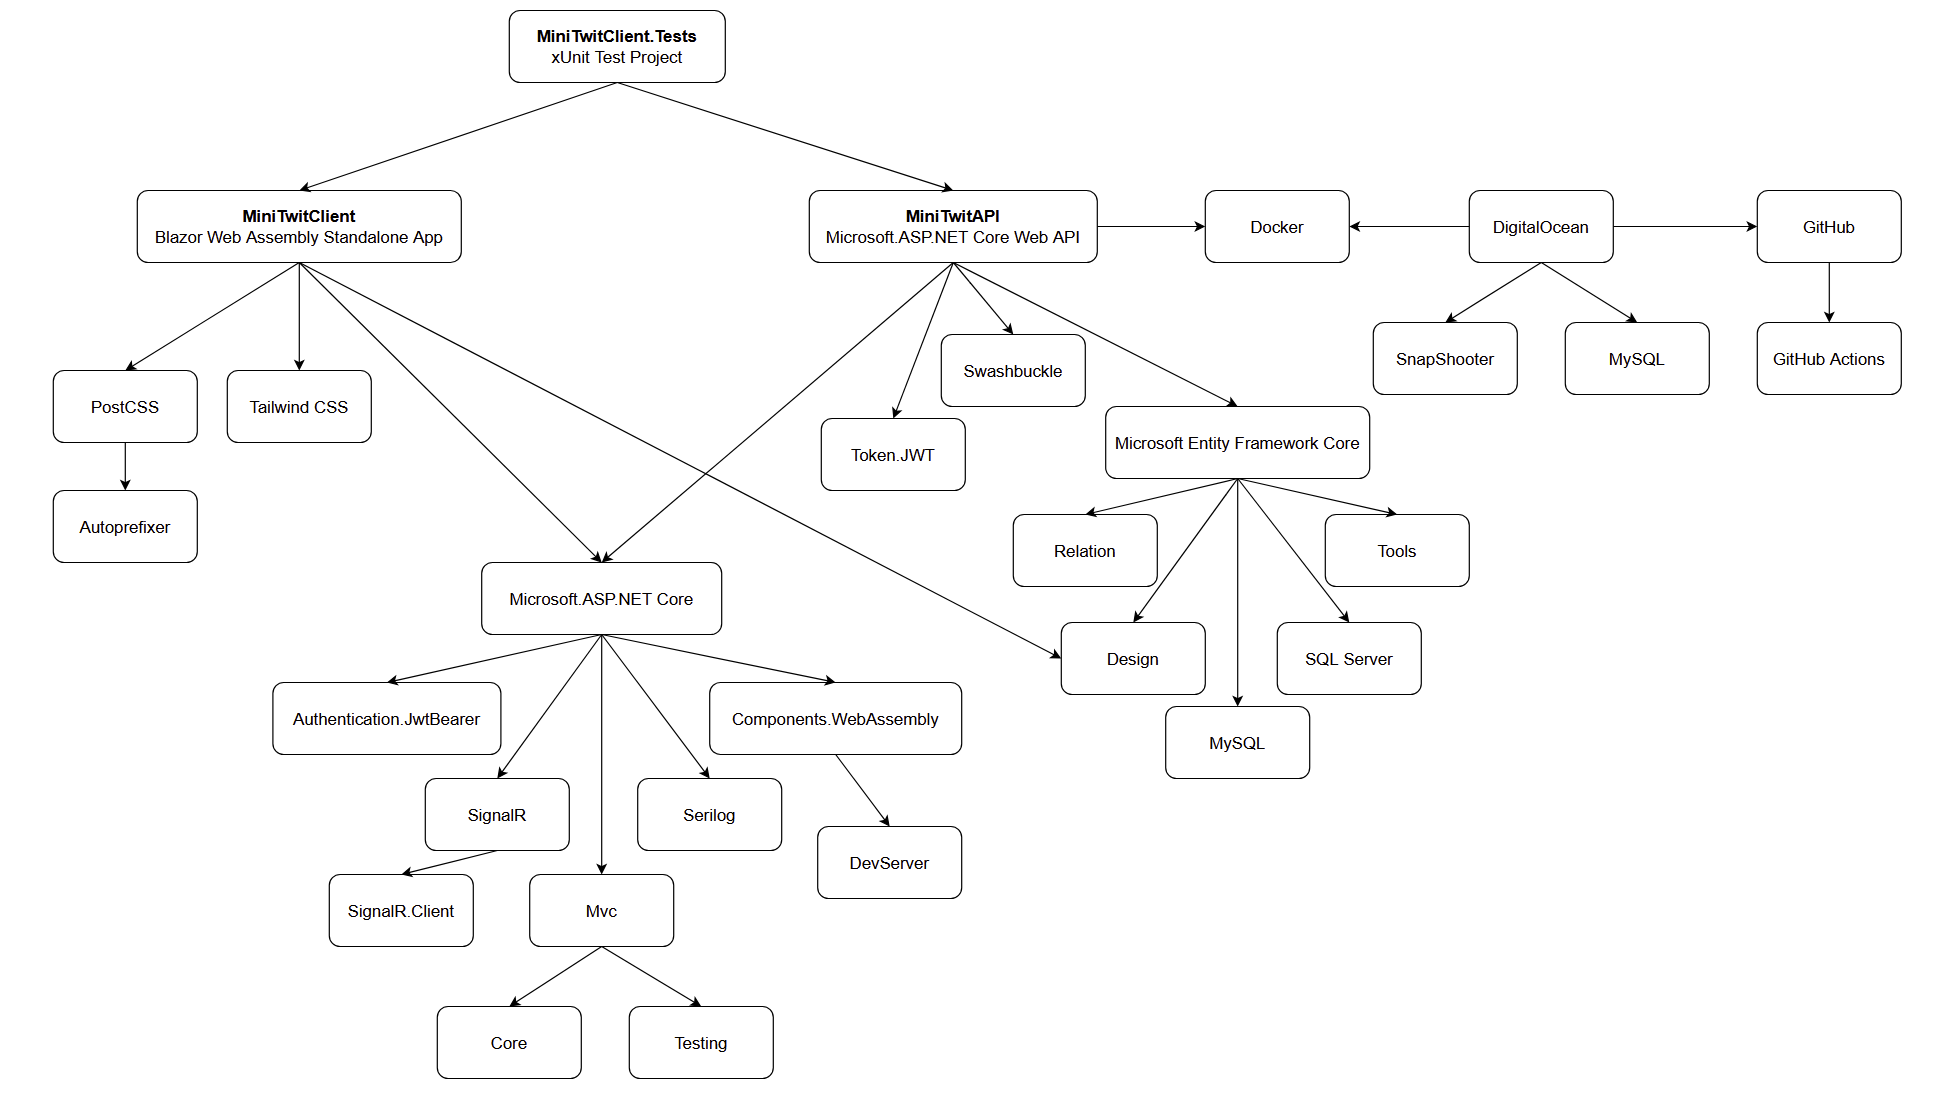
\includegraphics[width=1\linewidth]{images/DependecyDiagram.png}
    \caption{Dependency diagram of the entire system.}
    \label{fig:DependencyDiagram}
\end{figure}